\documentclass[11pt,varwidth=\maxdimen]{standalone}
%\documentclass{article}
\usepackage[english]{babel}	
\usepackage[utf8]{inputenc}	% Allows for writing special charachters in the tex-file 

\usepackage{amsfonts,amsmath,amssymb,bm,mathrsfs,mathtools,dsfont} 	% Standard mathematics 

\newcommand{\braces}[1]{\left\lbrace #1 \right\rbrace}
\newcommand{\brackets}[1]{\left( #1 \right)}
\newcommand{\squarebrackets}[1]{\left[ #1 \right]} 
\newcommand{\angles}[1]{\left\langle #1\right\rangle}
\newcommand{\abs}[1]{\left\lvert #1 \right\rvert}
\newcommand{\norm}[1]{\left\Vert #1 \right\Vert}

\usepackage[dvipsnames,table]{xcolor}
\definecolor{rmp}{RGB}{41, 43, 133}
\definecolor{myblue}{rgb}{0.24, 0.36, 0.44}
\definecolor{mygreen}{rgb}{0.367, 0.473, 0.0}
\newcommand{\myBlue}[0]{RoyalBlue}
\newcommand{\myGreen}[0]{OliveGreen}
\newcommand{\myRed}[0]{OrangeRed}
\newcommand{\myYellow}[0]{Goldenrod}


\usepackage{tikz}
\usepackage[compat=1.1.0]{tikz-feynman}
\usetikzlibrary{positioning,shapes,calc,arrows.meta}
\newcommand{\coord}[4]{({(#1)+(#3)*cos(#4)},{(#2)+(#3)*sin(#4)})}


\newcommand{\sscript}[1]{{\scriptscriptstyle \mathrm{#1}}}
\newcommand{\EFT}{\sscript{EFT}}


% % % % % % Commands % % % % % % %

\begin{document}

% Diagram 1
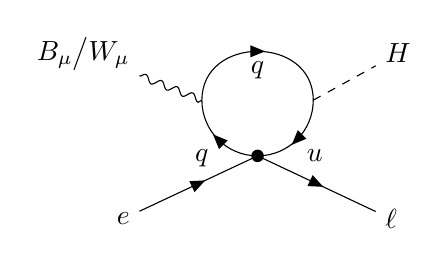
\begin{tikzpicture}
%\tikzset{baseline=(c.base)}
\tikzfeynmanset{inline=(c.base)}
\begin{feynman}
	\vertex (c);
    \node[circle, fill, inner sep=1.6pt] (aux) at (c);
    \vertex[above left=1cm of c] (l1);
    \vertex[above right=1cm of c] (l2);
    \vertex[below=0.8cm of c] (aux);
    \vertex[above=1.3cm of c] (aux2);
    \vertex[left=1.5cm of aux] (i) {$e$};
    \vertex[right=1.5cm of aux] (f) {$\ell$};
    \vertex[left=1.5cm of aux2] (i2) {$B_\mu \big/ W_\mu$};
    \vertex[right=1.5cm of aux2] (f2) {$H$};
    
    \diagram*[baseline=(c.base)] {
      {[edges=fermion]
        (c) -- [quarter left, edge label=$q$] (l1) -- [half left, edge label'=$q$] (l2)  -- [quarter left, edge label=$u$] (c),
        (i) -- (c) -- (f),
      },
      (i2) -- [boson] (l1),
      (l2) -- [scalar] (f2),
    };

\end{feynman}
\end{tikzpicture} 

\end{document}